\chapter{Introduction}

%============================= INTRODUCTION =================================
\section{Numerical Modeling of Magmas and state of the art}
\subsection{Motivation}
\lettrine{M}{agmatic} chambers are often thought as deep, distant and inaccessible systems. Subject to extreme conditions of pressure and temperature, the sole idea of physically approaching a magmatic chamber seems unrealistic and rather impossible, and in fact, it has never been done intentionally. However, in three separated and unrelated cases, magma has been drilled into accidentally, evidencing how little the scientific community really know about these systems, as well as defying the believes of them to be some sort of "black box", only approachable indirectly trough geophysical and geochemical methods. These cases are: Kīlauea volcano, Hawaii in 2005, when geothermal well KS-13, operated by the Puna Geothermal Venture intersected a molten magma body, of dacite composition, at 2.5 km depth (\cite{teplow2008}); Menengai caldera, Kenya in 2011 intersected several syenitic and trachytic magma bodies at depths of around 2 km (\cite{mbia2014}); and Krafla caldera, Iceland, when in 2009 the Icelandic Deep Drilling Project-1 (IDDP-1) intersected rhyolite magma at 2.1 km depth. This last case was particularly impactful given that Krafla is one of the most studied and well known volcanoes in Iceland, site of the most productive geothermal plant on the country, and intensely drilled into since it last eruption happened between 1975 and 1983 known as the Krafla Fires. The IDDP-1, an exploratory well operated mainly by Landvirskjun (the National Power Company of Iceland) was aiming to supercritical conditions of water, which had been estimated to be located at around 4 km depth. However, at 2.1 km, circulation was lost at the drilling bit, at the same time that rhyolite glass cutting were retrieved (\cite{elders2011}). It was then understood that a rhyolite magmatic body, of unknown size and shape, had been intersected. This magmatic body had not been detected by any geophysical survey carried out up to that date, and still remains unconstrained on shape and size. The cuttings retrieved from the drilling include quenched, rhyolitic glass and crystalline felsite, interpreted as the intrusion of a rhyolite melt into the surrounding felsitic rock (\cite{gautason2010}, \cite{schiffman2014}). However, the origin of the magmatic body is still under debate, and topic of a large scientific production. Some suggest that the magma encountered in IDDP-1 can be originated by the ascension of a melt produced by high degrees of partial melting of a rock of quartzofeldspathic composition at depth likely hydrothermally altered basalt, that then produces low partial melting of the shallower, host felsite, ultimately aided by hydrothermal fluids circulation (\cite{zierenberg2013}, \cite{masotta2018}, \cite{saubin2021}). Other theories say that this melt could have been emplaced during the last eruption taken place in this area, the Krafla Fires in 1975-1984 (\cite{axelsson2014}, \cite{eichelberger2020}). The absence of extensive crystallisation at the rooftop of the magma body, with an estimated temperature of 900°C (\cite{elders2011}, \cite{zierenberg2013}), evidenced that, against the common believe, magmatic bodies can stay melted at extremely shallow depths, thus raising the question of how and for how long can these bodies remain melted in the shallowest crust, and how can they be related to the deeper magmatic systems. Although this encounter did, in fact, allow scientist to just so slightly peek into in-situ magma, the finding was absolutely fortuitous, and replicating this occurrence, as well as properly benefiting from it from an economical and scientific point of view, it is not yet possible with the current available technology. Significant uncertainties persist regarding the shape, size, spatial distribution and temporal extent of cooling, as well as the exact response of the magma to the actual drilling. Hence, we still need to rely on the previously mentioned approaches to learn more about volcanic plumbing systems.

As can be easily inferred from what has been previously mention, understanding magmatic chambers and volcanic plumbing systems has always been an enormous challenge for volcanologist since this systems are extremely complex, heterogeneous, and constantly evolving. Characterized by diverse rheologies and transient conditions, they are largely inaccessible to direct observation. Thus, these systems are generally studied trough indirect observations that are produced by geophysics, geochemistry, used to study the Earth's interior in several different ways, and physical volcanology and igneous petrology, which interprets the deep volcanic and plutonic systems as causing agents of the volcanic phenomena that we observe on the surface, such as volcanic eruptions, volcanic deposits, and the plutonic provinces that outcrop all around the world. While these approaches give us extremely valuable information about magmatic processes, they are unavoidable constrained to high doses of interpretation and limited by the capabilities to the available technology, or by the quality of the found outcrops, and can, in some cases, fall short or insufficient to detect fundamental features of mentioned systems, or even the systems at all like in the three magma encounters. Reality is, none of these approaches really dwells into the real-time dynamics of magmatic chambers. However, there is one other method that allow us to have some approximate insight into what is possibly occurring inside these magmatic bodies, and this is numerical modeling, and more precisely, computational fluid dynamics. Thanks to numerical tools we can simulate a wide range of processes, mostly inaccessible in nature, but only partially approachable empirically in the laboratory, such as magma crystallization; and observable in nature, such as ash plume dispersion into the atmosphere.

Computational fluid dynamics (CFD) is a branch of fluid mechanics that, utilizing numerical methods and algorithms, solves fluid flows problems. By running numerical simulations of the different fluid phases involved, CFD are able to predict, at least to some extent, the motion of the fluid in complex scenarios that are often difficult or impossible to observe in nature, or to replicate experimentally. 

Coinciding with the development of digital computers, the origin of CFD can be traced back to the mid-20th century, strongly driven by the need to solve the Navier-Stokes equations, the fundamental nonlinear partial differential equations that describe fluid motion. With the evolution and increasing computational power of modern computers, CDF have evolved from more simple algorithms to highly sophisticated models able to simulate turbulent flows, multiphase and multi-component flows, heat transfer and chemical reactions, among other processes. A considerable effort has been made by engineers on further developing  CFD codes and algorithms born from the quick technological and industrial development of the modern world in the last two centuries. Key applications of CFD are predicting aerodynamic forces, optimizing airfoil shapes, simulating turbulence around aircraft, and analyzing thermal protection systems in spacecrafts on aerospace engineering; designing fuel-efficient vehicles, modeling engine combustion, evaluating ventilation and cooling systems, and improving aerodynamics on automobile engineering;  assessing wind loads on buildings and bridges, modeling urban airflow, predicting flood and sediment transport, and simulating air and water pollution on civil and environmental engineering;  optimizing performance in gas turbines, boilers, nuclear reactors, and wind and hydroelectric turbines on energy systems engineering; simulating blood flow in arteries and veins, airflow in respiratory systems, and targeted drug delivery in biomedical engineering and weather prediction, climate modeling, oceanography, and volcanic plume simulation, where large-scale fluid behavior interacts with heat, chemistry, and topography, on meteorology and geology.

Focusing on geological CFD software, some programs have being developed within the frame of geological and geothermal exploration, and few have being developed with the focus on magmatic systems. The development of software is often driven by volcanic risk assessment, resulting in programs with a strong focus on the eruptive processes such as pyroclastic density currents, like TITAN2D (\cite{titan2d2005}) or VOLCFLOW (\cite{volcflow}), and ash plumes evolution and dispersions such as ASH3D-A (\cite{mastin2013}) and FALL3D (\cite{costa2006}). However, there is a noticeable lack of commercial and accessible software specifically designed to simulate magmatic chamber processes, accounting for all the phases that constitute a magma, such as melt, crystals and volatiles dissolved in the melt or exsolved in the gas phase. Often, numerical simulations of magma dynamics are performed with specific modules developed for larger software, like MagmaFOAM for OpenFOAM (\cite{magmaFOAM2022}) or CFD module of COMSOL Multiphysics® commercial software.  \cite{dufek2005}, \cite{ruprecht2008}, \cite{dufek2010}, \cite{molina2012}, among others, have implemented different modifications on the multiphase code MFIX (\cite{syamlal1993}) in order to simulate several magmatic processes, that include crystals or bubbles bearing magmas, conduit dynamics for rhyolitic eruptions, cooling magmatic bodies and isothermal gas-driven magma mixing. Some noticeable studies exist with self-written, published or unpublished code: \cite{gutierrez&parada} present a quite complete multiphase model applied to a long-living and cooling basaltic magmatic reservoir. They account for different mineral species with variable crystal size, as well as $H_2O$ in the gas phase formed by variable sized bubbles, and present a detailed space-time distribution for the different phases formed during the cooling of the magmatic body.
\cite{simakin2012, simakin2022} developed a model to simulate convective melting in magmatic bodies with high-silica, wet and dry melts with a multiphase approach.

The motivation of this work comes from the need of having a better insight on the magma dynamics inside the chamber under conditions in which magma was not believed to be able to exist in a molten state without erupting. Thus, along this thesis, we aim to constrain the dynamics and thermo-mechanical properties of this shallow magmatic body while cooling, paying particular attention to the evolution of the magma when introducing its internal dynamics. For this, we will make numerical simulations of the thermo-fluid dynamics of the magma involved, to define the stability conditions for the different gas, liquid and solid phases at the Krafla volcano, and for rhyolitic magmas in general.

\subsection{Objective}
As numerical software continuous to evolve, so do the number of problems which scientist aim to resolve with said software. In many cases, the specificity of the problem requires advanced and personalized development that can be hard to achieve with commercial numerical software, which often develops solvers for more general problems. This could be a first explanation to why many scientific groups from research institutions all around the world tend to develop their own in-house software with applications on their specific problem. In the present work, we further develop GALES (\cite{garg2022}), the open source numerical simulation software that has been develop for many years in INGV Pisa, which solves the 4D dynamics of multi-component fluids in geometrically complex domains, using time-discontinuous stabilized space-time finite element method, parallelized and written in C++. We develop a solver that is able to deal with the fluid dynamics inside magmatic chambers with varying conditions of temperature and pressure (e.g. a cooling magmatic body intruded under given conditions of pressure, temperature and melt composition including total water as well as carbon dioxide).

As it has just being ascertained, commercial software often limits user access to core functionality, making it difficult to implement complex equations of state, such as those required for vulcanological applications, incising once more in the importance of self development when working in complex, non-commercial problems. This is particularly relevant in the study of magma chamber dynamics, since magma must be treated as a multi component mixture consisting of liquid melt, dissolved and exsolved volatiles, and crystals. In the present work, the  thermodynamic quantities appearing in the governing physical laws are computed based on this multi-component mixture. The densities (as well as other physical properties, which will be discussed further in the text) of individual components (melt, dissolved gases, and exsolved volatiles and crystals) are evaluated using appropriate equations of state, and the overall mixture density is then derived from these. Viscosity is initially calculated for the liquid phase, with gas and crystal-phase effects incorporated subsequently. Several models are employed to estimate the relevant physical properties, many of which are challenging or impractical to implement within the constraints of commercial CFD software. Thus, in GALES overcomes these limitations by enabling the incorporation of user-defined, problem-specific constitutive relations tailored for volcanic systems. 

In this work, the new features developed within GALES serve the purpose of studding the evolution and dynamics of shallow magmatic bodies, with a particular focus on the Krafla caldera case. As it was previously addressed, the accidental encounter with liquid magma produced in the Krafla caldera, as well as the cases in Kenya and Hawaii, defy the common belief that magmatic bodies at shallow depths should either erupt or quickly crystallize, as the pressure and temperature are expected to  be relatively low in comparison with lower crustal depths, facilitating gas exsolution from the magma and unchaining crystallization. Two key lessons can be learned from these findings. First, the scientific community knows less that they thought they knew regarding the behavior of magma at shallow crustal depths, and second, current geophysical methods clearly fail to properly observe shallow features, as the Krafla magmatic pocket had passed completely unnoticed under many years of intense geophysical surveying in the caldera. Within this context we apply our newly applied numerical techniques to make simulations of the thermomechanical behavior of a magma with the composition of that found in Krafla, under the conditions in which it was encountered. However, neither the size or the shape of this magmatic body is yet known, and conditions of temperature, pressure as well as composition have only been partially assessed from the cuttings retrieved during the drilling of the IDDP-1 exploratory well. As we are only constrained by the computational requirements of the numerical simulations, we find ourselves in a good position of experimentation. Therefore, we present a number of simulations to try to account for as many conditions as possible. We simulate magma dynamics and evolution while cooling for a number of sizes that we think are reasonably small in volume so that they might have been overlooked by geophysics, as well a number of pressure and temperature conditions, and variable water and carbon dioxide amounts. We cover a range of possible conditions that are realistic for the Krafla caldera environment and setting, and asses the state of the magma after specific periods of time, while tracking the time evolution of the magma dynamics with crystallization and gas exsolution. We simulate the heat loss trough the boundary to the rocks surrounding and observe the thermal evolution of the initially imposed geothermal gradient, having an important insight of the influence of a hot body in the temperature distribution of the rocks that surrounds it.

A successful interpretation of the data extracted from the simulation can give valuable insight to new projects that might actively pursue drilling into magma with some added constrains on timescales of cooling and phase distribution. This information is essential, since numerically proving that magma may or may not be present can make a great difference on wether a project is, for example, successfully founded or not.

%\subsection{Thesis outline}
\subsection{State of the art}
A number of models have been developed to study de dynamics inside magma chambers. However, commonly, models need to be simplified, as the systems to be resolved are extremely complicated, with the interplay of numerous mechanisms, which translates in a strong nonlinearity of the processes. Typical assumptions are thermodynamic equilibrium, steady state, 1D or 2D approximations and the presence of just one exsolved phase (gas or crystals, but not both). This assumptions, whilst, on occasions, creating unnatural or unrealistic scenarios, are necessary to understand the fundamental processes that influence the dynamics of such complex systems. 
In this section, a brief review of some of the models available in the literature is presented, to better understand the parting point of the work. 

%Organize the state of the art by 
%Check deepak's for older models
% 1- MFIX models
% 2-Guitierrez & parada
% 3-Simakin 2012 y 2022
% 4-MagmaFOAM
% 5-Oleg's new paper

\section{Geological setting}\label{sec:i}
\subsection{Iceland}
Before dwelling into the topic of Krafla, it is most pertinent to give some overview of the more general geological setting and history of Iceland. 

The most accepted hypotheses for the origin of Iceland states that it can be traced back up to the mid Cretaceous, 130 million years ago, during last Pangaea cycle and the formation of the North Atlantic. This time was characterized by the development of mid-ocean ridges and the separation o continents. A large mantle plume formed beneath Greenland, which triggered extensive mantle upwelling (\cite{wolfe1997}; \cite{holbrook2001}; \cite{rickers2013}). This was the cause of the mid Cretaceous and the continental flood basalts along the Arctic Mendelev Ridge, Alpha Ridge and Ellesmere Islands (\cite{lawver1994}; \cite{johnston2000}; \cite{sigmundsson2006}). The last 60 million years are characterized by an overall migration towards the northwest to the North American plate, carrying Greenland, and the southeast migration of the Eurasian plate, being determinant to the location of the Iceland hot spot. This divergent plate boundary constitutes the Mid-Atlantic Ridge (MAR) and has been separating the Eurasian and North American plates at an approximate rate of 2 cm per year (\cite{sella2002}; \cite{geirsson2006}).

During the Eocene (56 to 34 million years ago) the rifting and consequent separation of Greenland and Norway was initiated on the now extinct Aegir Ridge, East of the Iceland plum track. Around 24 million years ago, Late Oligocene-Early Miocene the Aegir ridge became extinct with the continued declining of the large mantle plume's extension and temperature, and the spreading center shifted to the incipient Kolbeinsey ridge, located to the West and parallel to the Aegir ridge. About 24 million years ago, the Kolbeinsey ridge and its continuation to the south, the Reykjanes ridges, were centered over the hot spot (figure \ref{fig:NA_map}). Since then, the spreading center has moved a shifted in what is know as magmatic induced rift jumps (\cite{hjartarson2017}). Controlled by magma upwelling from the plume, the lithospheric crust can be thinned and develop a new ridge, shifting the spreading activity to a new axis (\cite{mittelstaedt2008}. These rift jumps explain the Reykjanes-Kolbeinsey ridge to have been moved 240 km northwest from the plume center. Consequently, the plume is now believed to be located under Vatnajökull, the larges glacier on Iceland (\cite{einarsson1991}; \cite{einarsson2001} \cite{holbrook2001}; \cite{sigmundsson2006}; \cite{foulger2006}).

\begin{figure}
    \centering
    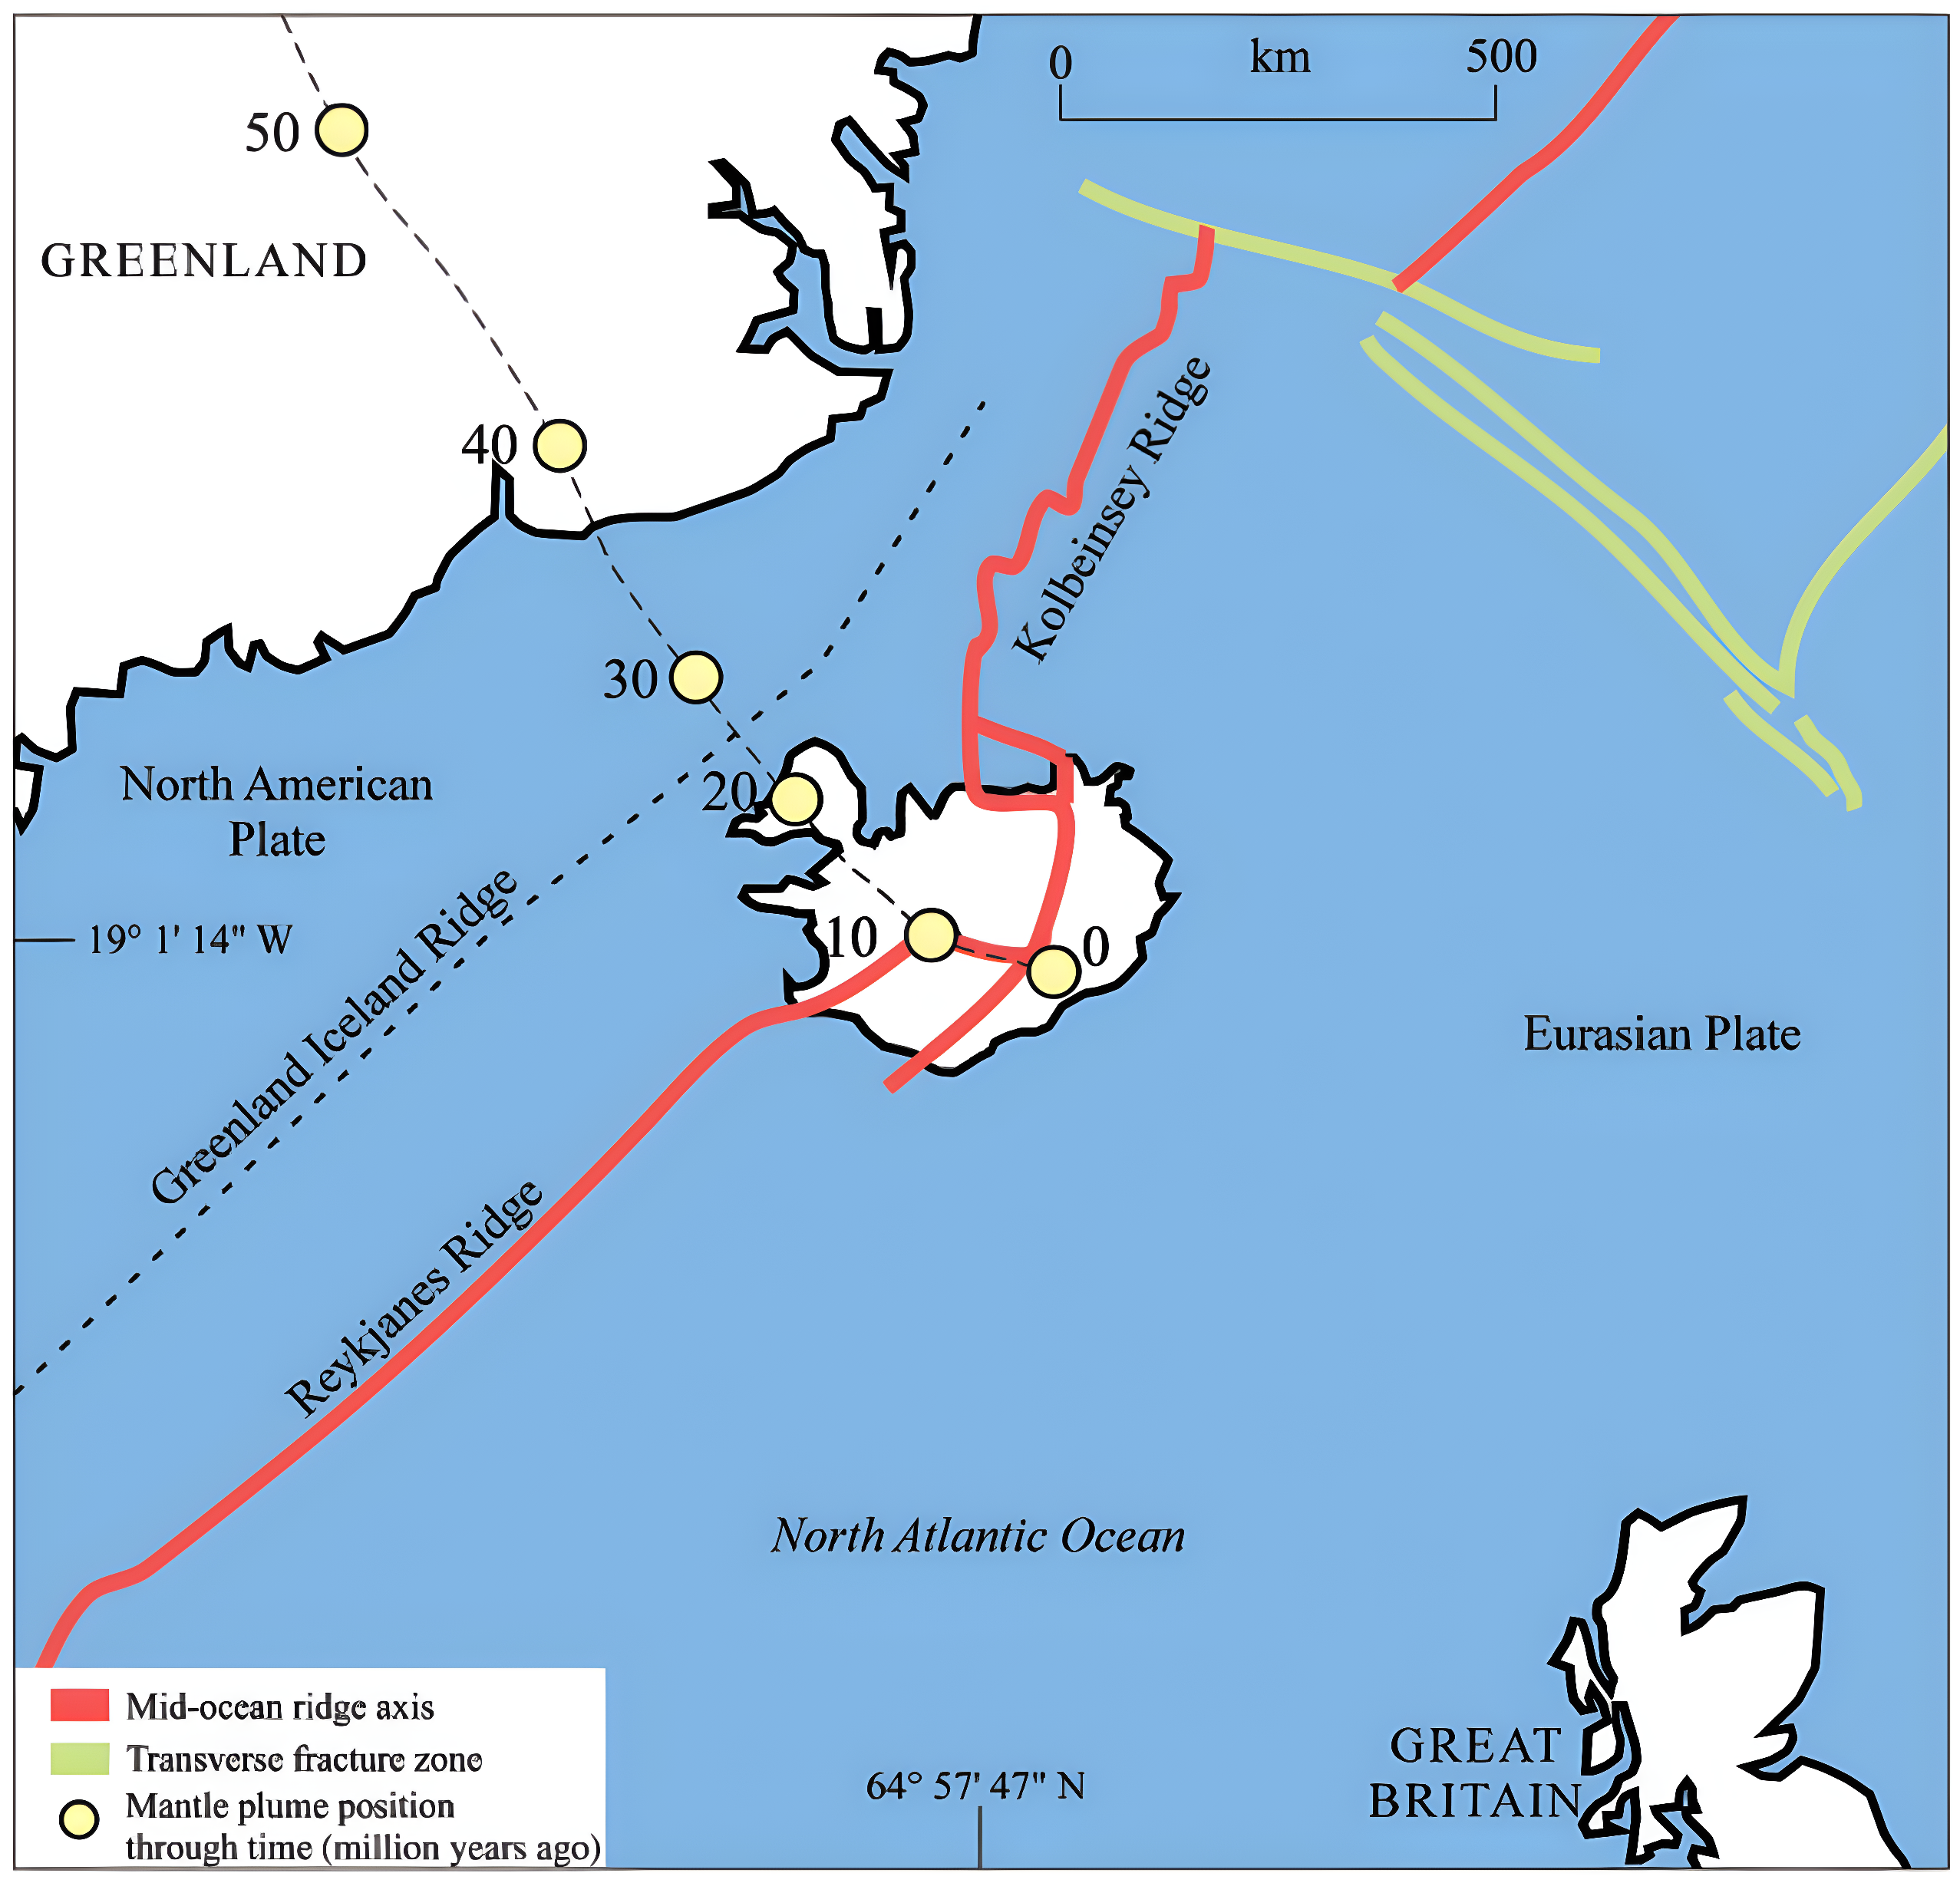
\includegraphics[width=1\linewidth]{img/chapter1/Ridges_map.png}
    \caption{\cite{fitton1997}}
    \label{fig:NA_map}
\end{figure}

The current tectonic setting of Iceland is controlled by the continued spreading of the Mid-Atlantic Ridge by the already mentioned subbranches: Kolberinsey Ridge (KR) in the north and the Reykjanes Ridge (RR) in the south. These ridges have formed two Icelandic microplates named Hreppar in the South and Tjörnes in the North. Three major neovolcanic zones can be differentiated since they concentrate the majority of the volcanic activity, faulting and deformation. These are: North Volcanic Zone (NVZ), East Volcanic Zone (EVZ) and West Volcanic Zone (WVZ). During the last 2-3 million of years has being the most active one. The NVZ and EVZ, are both aligned in the East of the island, located 100-150 km to the East of the main overall plate boundary, defined by the RR and the KR, and in a bigger scale by the Mid-Athlantic Ridge. This offset rift is connected to the RR in the south by the South Iceland Seismic Zone (SISZ), a seismologically active area that accommodates the offset between the West and the East Volcanic Zone, and to the northern KR by the Tjörnes Fracture Zone (TFZ). In the middle part of Iceland, the offset ridge of the East is linked to the Wester Volcanic Zone by the Mid-Iceland Belt (MIB), a perpendicular to the axis volcanic zone that joints with the EVZ and the NVZ beneath Vatnajökull (\cite{sigmundsson2006}). This tectonic configuration can be better understand in figure \ref{fig:iceland_map}.

\begin{figure}
    \centering
    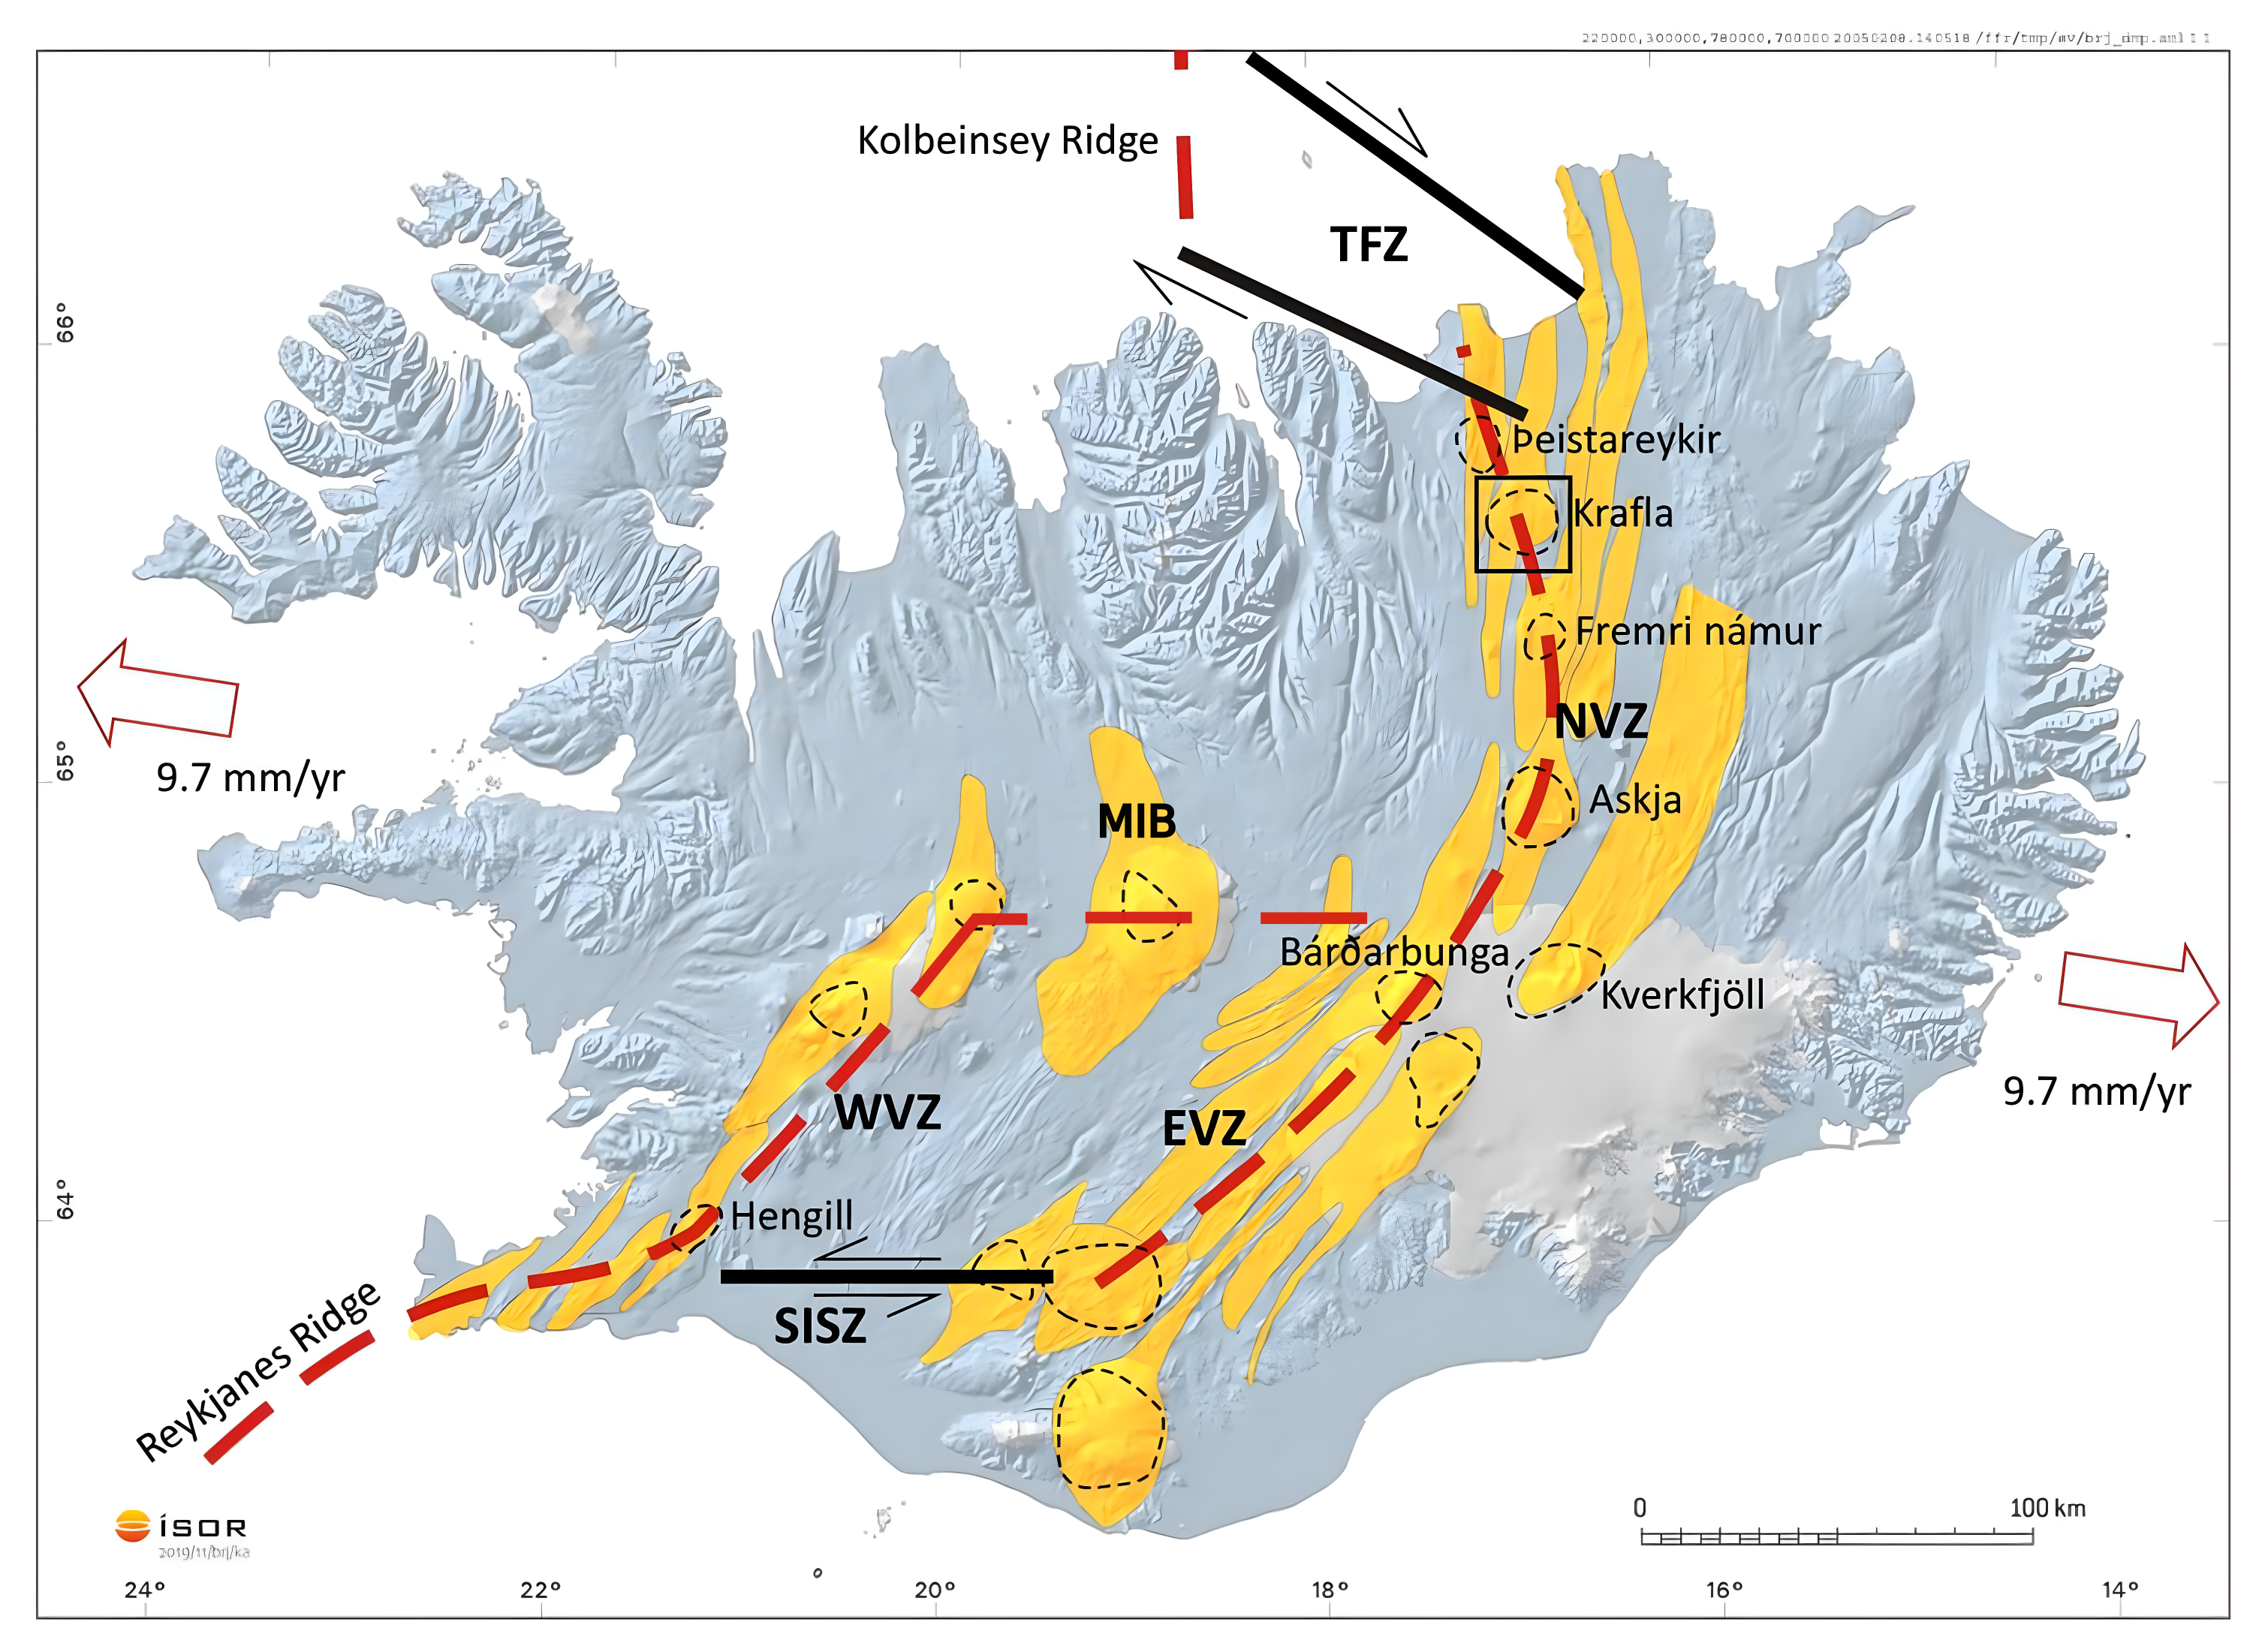
\includegraphics[width=1\linewidth]{img/chapter1/volcanic_zones.png}
    \caption{\cite{arnason2020}}
    \label{fig:iceland_map}
\end{figure}

The Northen Volcanic Zone has being active for the past 6-7 million years. The thickness of the crust in the axial zone is somewhere between 30 to 40 km, and decreases with the distance to the axis down to 20 to 30 km (\cite{björnsson1985}). This area is characterized by the presence of extensive and numerous fissure swarm, with a North-South orientation. Five main volcanic systems conform the area: Þeistareykir, Krafla, Fremrinámar, Askja, and Kverkfjöll.

\subsection{Krafla}
With the preceding overview of the Icelandic geological setting, we can focus our attention into de Krafla volcano. The Krafla volcanic system is a prominent geological feature located in the Mývatn region in the North of Iceland. Its geographical coordinates place its center at approximately 65°43'-65°44'N latitude and 16°47'W longitude. 

The Krafla volcano itself comprises two main structural elements: a central volcano and an associated fissure swarm. The central volcano forms a low, broad shield-like edifice, approximately 20-25 km in diameter. At the heart of the central volcano lies a distinct caldera, measuring approximately 10 km east-west and 8 km north-south. This caldera was formed during an explosive eruption 110 ka ago (\cite{sæmundsson1991}).
The fissure swarm constitutes an important tectonic feature in the area. With a direction of NNE-SSW, and with a length and width of approximately 80-100 km and 4-10 km respectively intersects the caldera, accommodating the major part of the Northern Volcanic Zone crustal spreading in this area. These features can be appreciated in the map portrayed in figure \ref{fig:krafla_map}.

Krafla stands out as one of Iceland's most significant and intensely studied volcanic systems due to its rich eruptive history, including the historical Mývatn Fires (1724-1729, 1746) and the instrumentally monitored Krafla Fires (1975-1984). This last eruption, in particular has provided the scientific community with invaluable data on the behavior of rift zones during active periods. The Krafla Fires represented an unprecedented opportunity for geoscientists to observe and measure volcanic processes such as magma accumulation, dike intrusion, crustal deformation, and eruption in near real-time. This episode significantly advanced the understanding of volcanism in extensional rift settings.
Furthermore, Krafla hosts a powerful high-temperature geothermal system that has been exploited for energy production for decades. This practical application necessitates detailed subsurface investigation, contributing a wealth of drilling data, temperature measurements, and fluid chemistry information that complements surface geological and geophysical studies.

\begin{figure}
    \centering
    \includegraphics[width=1\linewidth]{img/chapter1/Krafla_1.png}
    \caption{\cite{masotta2018}}
    \label{fig:krafla_map}
\end{figure}

\subsubsection{Volcanic history}
The main structure in the Krafla systems is its caldera, formed around 110000 years ago, during the Eemian interglacial period after a phreatic, dacitic eruption took place, and was followed by two other silicic or semi-silicic eruptions, on 80 ka ago, forming the edifices of Hlíðarfjall to the Southwest of the caldera, Jörundur to the East-Southeast and Rani to the Northwest (\cite{sæmundsson1991}) This volcanism might have formed a inner caldera, now buried by more recent deposits (\cite{arnason2020}). Subglacial eruptions produced characteristic hyaloclastite ridges aligned with the fissure swarm trend within the caldera. Notable examples include the Mt. Krafla itself, which may represent a resurgent dome formed after the caldera collapse (\cite{castillo2021}). 24 ka ago a subglacial fissure eruption formed the obsidian ridge in the Southeastern are of the caldera known as Hrafntinnuhryggur. Alternating with these eruptions, the volcanic activity is dominated by basaltic fissure eruptions an dyke injections.

In the post-glacial era, about 8 ka ago, the spreading shifted from the East to the West of the fissure swarm, although volcanic activity didn't increase during this period. Just one noticeable phreatic eruption took place, at about 5 ka years ago, forming the Hvannstóð crater, in the Northwestern part of the main caldera. 3 ka years ago, the spreading moved back to the East, and since then, eruptions have occur every 300-1000 years (\cite{sæmundsson1991}). During both of these periods the volcanic activity was concentrated, with very few exceptions, on the eastern side fissure swarm due to a 18° difference on the opening directions of the East-side crust of the swarm, between the southern part from the caldera (with an approximate direction of 22°SE) and the northern part (with a direction of 4°SE approximately), according to (\cite{drouin2017}). This may have led to a N-S opening component, favoring magma ascent of magma (\cite{arnason2020}).

The last two eruptive episodes have occurred during historical times: the Mývatn Fires (1724-1729) and the Krafla Fires (1975-1984).

\subsubsection{Mývatn Fires (1724-1729)}
The Mývatn Fires started when a phreatomagmatic eruption occurred inside the caldera, forming the characteristic Víti crater on the 17th of May, 1724 (see the exact location of the crate in figure \ref{fig:krafla_map}). The eruption is believed to have been triggered by the intrusion of rhyolitic magma into the hydrothermal system (\cite{montanaro2021}). The main center of the activity moved towards Leirhnjúkur, situated 2 km West from Víti, with repeated dyke injections into the fissure swarm. In 1727 the peak activity commenced with effusive basaltic fissure eruptions around the area. Two main fissure eruptions occurred between 1727 and 1729 within the caldera, although there is record of a smaller eruption taking place west of Námafjall (\cite{sæmundsson1991}).

\subsubsection{Krafla Fires (1975-1784)}
The Krafla fires is the most recent eruption of the Krafla volcano. This eruptive period is exceptionally significant because it was the first such episode on a mid-ocean ridge segment to be extensively monitored using modern geophysical techniques, providing unprecedented insights into rift dynamics. The episode began in December of 1975 with a small and brief basaltic fissure eruption north of the Leirhnjúkur ridge within the caldera, preceded by an intense earthquake swarm.

It was characterized by repeated episodes of inflation and deflation. The inflation periods, lasting from months to over a year, were interpreted as magma accumulating in a shallow reservoir located approximately 3 km beneath the surface. Seismic studies using S-wave attenuation and P-wave delays supported the presence of a melt-bearing body at depths of 3-7 km (\cite{einarsson1978}). These S-wave "shadows", named as in \cite{arnason2020} can be seen in figure \ref{fig:krafla_map} as the gray-colored shapes referred as inferred magma chamber on the map's legend. The maximum rate of magma inflow into this reservoir during inflation was estimated at 5 m³/s. The rapid deflation events, typically lasting from a day to several months 31, corresponded to the failure of the magma reservoir walls and the lateral injection of magma as dikes into the NNE-SSW trending fissure swarm (\cite{einarsson1980}). In total, 9 of these inflation and deflation episodes actually ended up erupting, with the final eruption of the Krafla Fires taking place in September 1984. A detailed study of the ground deformation during and after this eruption (\cite{tryggvason1986}) suggests that deeper magma reservoirs feed shallower ones, at approximately 2.6 km depth, an idea that partially support the previously mentioned S-waves "shadows" as melt-bearing bodies at depths between 3 and 7 km. The average opening across the 70-80 km affected rift segment has been estimated at 4.3-5.4 meters (\cite{hollingsworth2012}). 

Recent detailed petrological analysis of the lavas erupted during the Krafla Fires has revealed a more complex magmatic system than previously assumed based solely on geophysics (\cite{rooyakkers2024}). Evidence indicates the simultaneous tapping of two distinct basaltic magma reservoirs during several eruptions: a primitive magma sourced from the lower crust (~14-19 km depth) and a more evolved tholeiitic magma from the shallower reservoir system (~7-9 km depth, likely encompassing the 3 km seismically-imaged chamber). Mixing between these two magma types occurred near the northern caldera margin. This implies rapid magma ascent pathways from the lower crust that potentially bypassed the main shallow storage zone, suggesting a decoupling of flow paths and hydraulic connection between reservoirs at different crustal levels during the rifting process and simultaneous feeding of the eruptions in several events.

\subsubsection{Geothermal System}
As previously mentioned, Krafla hosts a high-enthalpy geothermal system located in the center the outer caldera, which provides a geothermal power plant with a production capability of 60 MW. 
A total of 43 wells have been drilled inside the caldera for exploration and production purposes. Some of the wells have also being used for reinjection. Analizeing the well formation temperature from the drilling logs, \cite{mortesen2015}, \cite{arnason2020}, \cite{scott2022} and reference therein suggest the presence of five distinct subfields withing the caldera: Leirbotnar-Vítismór and Suðurhlíðar located west and east of the Hveragil fissure; Hvíthólar on the southern rim of the caldera and Vestursvæði and Sandabotnaskarð, located to the north and south of Suðurhlíðar respectively. 
Leirbotnar-Vítismór subfield is characterized by the presence of an isothermal layer between 500 and 1000 m b.s.l. at 200°C, interpreted as a low permeability aquitard (Bodvarsson, Pruess, et al., 1984; Stefánsson, 1981). This aquitard separates separates the sub-boiling upper reservoir from the underlying two phase zone, which follows the boiling curve with depth.


\subsubsection{Current status}
At present times and moment of production of this thesis, the Krafla volcano is generally considered to be in a state of quiescence following the end of the Krafla Fires in 1984, although ongoing processes related to post-rifting adjustment and geothermal activity continue. 

\subsection{Icelandic Deep Drilling Project - 1}

%============================= SECTIONS =================================

